

\documentclass[12pt]{extarticle}

\usepackage{summary-intro}


\begin{document}



\sumintro{Time Travel}{Spring 2023}

\section{Defining Time Travel}

\emph{Our working definition:} to travel in time is for there to be a discrepancy between: 

\begin{enumerate}
\item the start-time and end-time of one's journey (\textit{external time}), and

\item the duration of the journey from one's own perspective (\textit{personal time}).

\end{enumerate}

\section{Inconsistent Time Travel Stories}

For a time travel story to be consistent is for it to never make conflicting statements about what the world of the story is like at a given time.

\begin{itemize}
\item For instance, \emph{Back to the Future} is  an inconsistent time travel story:

\end{itemize}
 \begin{center}
    \begin{tabular}{l|l}
      \textbf{What we're told} & \textbf{When we're told} \\
      \hline
      In 1985, George is unhappy & beginning of film\\
      In 1985, George is happy & end of film\\
    \end{tabular}
  \end{center}

\subsection{Caveat: No ``Changing Timeline'' Stories}

``Changing Timeline'' stories rely on two different senses of time:


\begin{enumerate}

\item an ordinary notion of time, which is used to describes changes \emph{within} a given timeline;
\item a non-ordinary sense of time, which is used to describe ``changes'' in the timeline itself.

\end{enumerate}
\emph{But}: is the second sense really intelligible?




\begin{figure}
\begin{center}
\begin{tikzpicture}[scale = 0.65]
\draw[->] (0,0) -- (0,8); % time axis
\draw[->] (0,0) -- (8,0); % space axis
\node at (3.25,-1.5) {\small \emph{super time}}; % space label
\node at (-0.4,4) {\small \rotatebox{90}{\emph{ordinary time}}}; % time label



\draw[ultra thick] (2,0) -- (2,7.8); % original timeline
\node at (2,-0.3) {\scriptsize \emph{timeline}}; % label
\node at (2,-0.61) {\scriptsize \emph{``before''}}; % label
\node at (2,-0.84) {\scriptsize \emph{change}}; % label

\draw [black, ultra thick] (2,6.5) circle [radius=0.04]; %happy point
\node at (2.6,6.9) {\tiny \emph{George}}; % top label
\node at (2.6,6.7) {\tiny \emph{unhappy}}; % bot label

\draw[ultra thick] (4.5,0) -- (4.5,1.5); % modified timeline
\draw[ultra thick, snake]  (4.5,1.5) -- (4.5,7.8); % modified timeline
\node at (4.5,-0.3) {\scriptsize \emph{timeline}}; % label
\node at (4.5,-0.61) {\scriptsize \emph{``after''}}; % label
\node at (4.5,-0.84) {\scriptsize \emph{change}}; % label

\draw [black, ultra thick] (4.5,6.5) circle [radius=0.04]; %unappy point
\draw [black, ultra thick] (4.5,6.4) -- (4.5,6.6) ; %supplementary line
\node at (5.2,6.9) {\tiny \emph{George}}; % top label
\node at (5.2,6.7) {\tiny \emph{happy}}; % bot label



\draw [dotted, thick] (0,6.5) -- (8,6.5);% 1985 line
\node at (-0.5,6.5) {\scriptsize \emph{1985}}; % label


\draw [dotted, thick] (0,1.5) -- (8,1.5);% time t line
\node at (-0.5,1.5) {\scriptsize \emph{1955}}; % label

\end{tikzpicture}
\end{center}
\caption{A change in George's timeline. The straight lines represent events as they ``originally'' occurred. The jagged line represents events as they occur ``after'' the change.}
\label{f-george}
\end{figure}





\subsection{Caveat: No World Travel Stories}

One can make some inconsistent time travel stories consistent by interpreting them as world travel stories. 

\vspace{3mm}
\noindent
\emph{But:} that just means that we've changed the subject.


\section{The Grandfather Paradox}


You travel back in time to kill your grandfather, who is yet to have any children. You have a loaded gun at point-blank range. 

\begin{itemize}

\item If you succeed, Grandfather will never have any children. So you'll never be born, which contradicts the setup of the story.

\item If you don't succeed, what stops you?


\end{itemize}
Some reasons you might think the Grandfather Paradox is interesting:

\begin{enumerate}

\item It may show that the concept of time travel is incoherent.

\item It raises questions about whether the laws of physics could rule out paradoxical time travel in a principled way, without banning it altogether.

\item It may show that time travel is incompatible with free will.


\end{enumerate}
%(For what it's worth: I think these reasons are all mistaken.)


\section{A Toy Model\footnote{This model is due to philosophers Frank Arntzenius and Tim Maudlin.}}

The particles of our world live on two dimensions and obey the following laws:
\begin{description}
\item[Law 1]  In the absence of collisions, a particle's velocity remains constant.


\item[Law 2] When two particles collide, they exchange velocities. (There are no collisions involving more than two particles.)

\end{description}

\subsection{Wormholes}
Our laws are consistent with wormholes. For instance:

\begin{figure}[ht]
\begin{center}
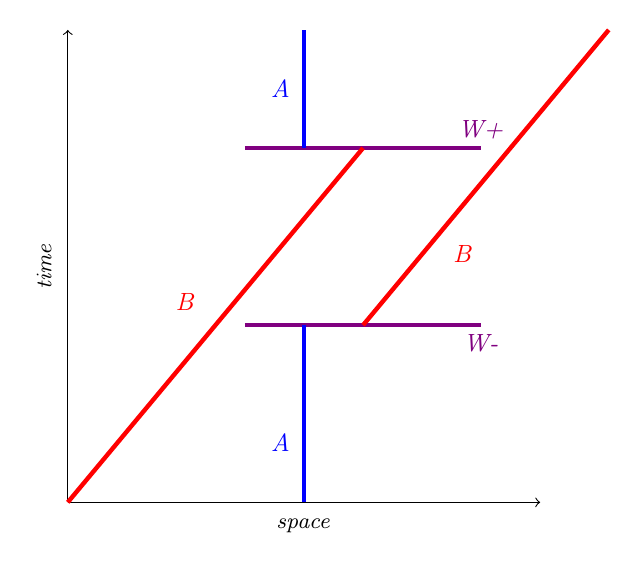
\begin{tikzpicture}[scale = 0.75]
\draw[->] (0,0) -- (0,8); % time axis
\draw[->] (0,0) -- (8,0); % space axis
\node at (4,-0.4) {\footnotesize \emph{space}}; % space label
\node at (-0.4,4) {\footnotesize \rotatebox{90}{\emph{time}}}; % time label

\draw[ultra thick, violet] (3,6) -- (7,6); % Line W+
\node[violet] at (7,6.3) {\small \emph{W+}}; % W+'s label
\draw[ultra thick, violet] (3,3) -- (7,3); % Line W-
\node[violet] at (7,2.7) {\small \emph{W-}}; % W-'s label

\draw[ultra thick, blue] (4,0) -- (4,3); % A's timeline, part 1
\node[blue] at (3.6,1) {\small \emph{A}}; % A's label, part 1
\draw[ultra thick, blue] (4,6) -- (4,8); % A's timeline, part 2
\node[blue] at (3.6,7) {\small \emph{A}}; % A's label, part 2
%\node at (4,3.3) {\footnotesize $p$}; % p label
%\node at (4,5.7) {\footnotesize $p$}; % p label


\draw[ultra thick, red] (0,0) -- (5,6); % B's timeline, part 1
\node[red] at (2,3.4) {\small \emph{B}}; % B's label, part 1
\draw[ultra thick, red] (5,3) -- (9.16,8); % B's timeline, part 2
\node[red] at (6.7,4.2) {\small \emph{B}}; % B's label, part 2
%\node at (6,6.4) {\footnotesize $p'$}; % p label
%\node at (6,2.6) {\footnotesize $p'$}; % p label



\end{tikzpicture}
\end{center}
\label{f-wormhole}
\end{figure}

In this diagram, the points represented by \emph{W-} are identified with the points represented by \emph{W+}. $A$ jumps to the future when its spacetime trajectory reaches a point at which the wormhole is active; $B$ jumps to the past when its spacetime trajectory reaches a spacetime point at which the wormhole is active.


\subsection{A Toy Version of Grandfather's Paradox}


\begin{figure}[ht]
\begin{center}
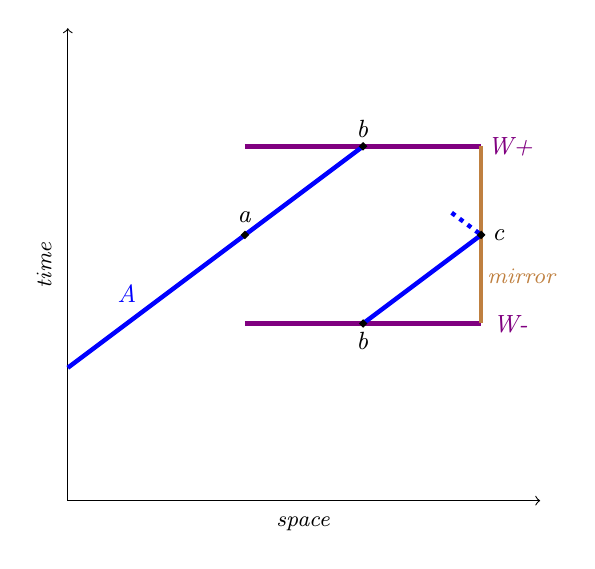
\begin{tikzpicture}[scale = 0.75]
\draw[->] (0,0) -- (0,8); % time axis
\draw[->] (0,0) -- (8,0); % space axis
\node at (4,-0.4) {\footnotesize \emph{space}}; % space label
\node at (-0.4,4) {\footnotesize \rotatebox{90}{\emph{time}}}; % time label

\draw[ultra thick, violet] (3,6) -- (7,6); % Line W+
\node[violet] at (7.5,6) {\small \emph{W+}}; % W+'s label
\draw[ultra thick, violet] (3,3) -- (7,3); % Line W-
\node[violet] at (7.5,3) {\small \emph{W-}}; % W-'s label

\draw[ultra thick, brown] (7,3) -- (7,6); % mirror
\node[brown] at (7.7,3.8) {\footnotesize \rotatebox{0}{\emph{mirror}}}; % mirror's label

\draw[ultra thick, blue] (0,2.25) -- (5,6); % A (1)
\node[blue] at (1,3.5) {\small \emph{A}}; % label
\draw[ultra thick, blue] (5,3) -- (7,4.5); % A (2)
\draw[ultra thick, blue, dotted] (6.5,4.875) -- (7,4.5); % A (3)

\draw [black, ultra thick] (3,4.5) circle [radius=0.02]; %point a
\node at (3,4.8) {\small \emph{a}}; % label

\draw [black, ultra thick] (5,6) circle [radius=0.02]; %point b (1)
\node at (5,6.3) {\small \emph{b}}; % label

\draw [black, ultra thick] (5,3) circle [radius=0.02]; %point b (2)
\node at (5,2.7) {\small \emph{b}}; % label

\draw [black, ultra thick] (7,4.5) circle [radius=0.02]; %point c
\node at (7.3,4.5) {\small \emph{c}}; % label


\end{tikzpicture}
\end{center}
\label{f-toy}
\end{figure}

Particle $A$ is on a ``paradoxical path''. It travels rightward, passes through spacetime point $a$ and enters the wormhole at spacetime point $b$, jumping to the past. It exits the wormhole and continues its rightward trajectory until it reaches the mirror at spacetime point $c$. But what happens next? 

\subsection{An answer to the toy paradox}

\begin{itemize}

\item One does not characterize a world by \emph{first} deciding how many particles the world is to contain (and assigning them each a position and velocity at a time), and \emph{then} using the dynamical laws to calculate the spacetime trajectories of these particles. 

\item Instead, one characterizes a world by \emph{first} drawing a family of spacetime trajectories that conform to the dynamical laws and \emph{then} using the laws to determine how many particles the resulting world must contain. 

\item So: it is a mistake to think that one can characterize a world by stipulating that it is to contain a single particle traveling as in figure~\ref{f-toy} and then ask what happens when the dynamical laws are used to calculate the particle's spacetime trajectory.


\end{itemize}


\section{The Grandfather Paradox}


Bruno travels back in time to kill Grandfather, who is yet to have any children. He has a loaded gun at point-blank range. 

\begin{itemize}

\item If Bruno succeeds, Grandfather will never have any children. So Bruno will never be born, which contradicts the setup of the story.

\item If Bruno doesn't succeed, what stops him?


\end{itemize}

\iffalse %repeats the earlier motivations for considering this paradox

\section{What Does the Paradox Show?}

Some possible answers:
\begin{enumerate}

\item It shows that the concept of time travel is incoherent.

\item It raises questions about whether the laws of physics could rule out paradoxical time travel in a principled way, without banning it altogether.


\item It shows that time travel is incompatible with free will.


\end{enumerate}
I think these answers are all mistaken!

\fi 



\section{What is Free Will?}

The following hypothesis is meant to capture the idea that someone who acts freely has \emph{control} over the action she performs:
\begin{description}
\item[Control Hypothesis]
An agent acts freely in doing $X$ if and only if: (1) she does $X$ by making a certain decision, and (2) she is in a position to do something other than $X$ by making a different decision.

\end{description}


\begin{itemize}
\item The Control Hypothesis is actually incorrect. But it is a good starting point for elucidating the connection between time travel and free will, so we'll treat it as our working hypothesis for now.

\item We'll assume the Control Hypothesis, and consider a couple of arguments purporting to show that Bruno fails to act freely because he was {not} in a position to make a different decision about how to take his shot.
\end{itemize}


\section{First Argument}

\emph{Argument:} We know that, on pain of contradiction, Bruno's assassination attempt will fail. So Bruno isn't free to pull the trigger.


\vspace{3mm}
\noindent
\emph{Reply:} It is important to distinguish between the following two questions:

\begin{itemize}

\item Whether we---who live in the present day---have information about Grandfather's future that entails Bruno's assassination attempt will fail. 

\item Whether Bruno was in a position to kill Grandfather, regardless of whether we---who live in the present day---happen to know that things won't actually turn out that way.

\end{itemize}




\section{Second Argument}

\emph{Argument:} If Bruno were ever on track to kill Grandfather, the laws of physics would intervene to derail him.



\subsection{Determinism}

For a system of laws to be \textbf{determinisitic} is for it to entail, on the basis of a full specification of the state of the world at any given time, a full specification of the state of the world at any later time. (If the laws are \textbf{reversible}, then we can evolve backwards from a full specification at a given time to a full specification at any earlier time.)

\begin{itemize}

\item \emph{Note:} Possessing free will is not simply a matter of having a decision-making process that is not subject to deterministic laws.


%\newpage

\item \emph{Note:} Two different conceptions of physical law are useful to focus on here:


\begin{enumerate}


\item \textbf{Regularity Conception}: The laws tell us what \emph{will} happen, on the basis of what has happened. The laws \textit{summarize} patterns of events (past through future). 

\item \textbf{Governing Conception}: The laws tell us what \emph{must} happen, on the basis of what has happened. The laws \textit{govern} or \textit{constrain} physical events. 


\end{enumerate}


\begin{center}
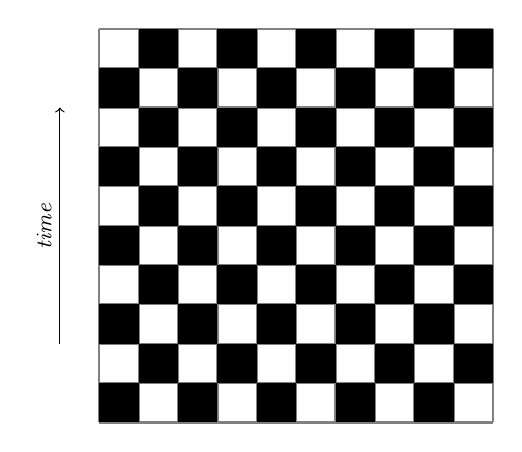
\begin{tikzpicture}[scale = 0.5]
\draw[step=1cm,gray,thick] (0,0) grid (10,10);

% Time arrow
\draw[->] (-1,2) -- (-1,8);
\node at (-1.4,5) {\footnotesize \rotatebox{90}{\emph{time}}}; % time label


%Row 0
\fill[black] (0,0) -- (0,1) -- (1,1) -- (1,0) -- cycle;
\fill[black] (2,0) -- (2,1) -- (3,1) -- (3,0) -- cycle;
\fill[black] (4,0) -- (4,1) -- (5,1) -- (5,0) -- cycle;
\fill[black] (6,0) -- (6,1) -- (7,1) -- (7,0) -- cycle;
\fill[black] (8,0) -- (8,1) -- (9,1) -- (9,0) -- cycle;

%Row 2
\fill[black] (0,2) -- (0,3) -- (1,3) -- (1,2) -- cycle;
\fill[black] (2,2) -- (2,3) -- (3,3) -- (3,2) -- cycle;
\fill[black] (4,2) -- (4,3) -- (5,3) -- (5,2) -- cycle;
\fill[black] (6,2) -- (6,3) -- (7,3) -- (7,2) -- cycle;
\fill[black] (8,2) -- (8,3) -- (9,3) -- (9,2) -- cycle;

%Row 4
\fill[black] (0,4) -- (0,5) -- (1,5) -- (1,4) -- cycle;
\fill[black] (2,4) -- (2,5) -- (3,5) -- (3,4) -- cycle;
\fill[black] (4,4) -- (4,5) -- (5,5) -- (5,4) -- cycle;
\fill[black] (6,4) -- (6,5) -- (7,5) -- (7,4) -- cycle;
\fill[black] (8,4) -- (8,5) -- (9,5) -- (9,4) -- cycle;

%Row 6
\fill[black] (0,6) -- (0,7) -- (1,7) -- (1,6) -- cycle;
\fill[black] (2,6) -- (2,7) -- (3,7) -- (3,6) -- cycle;
\fill[black] (4,6) -- (4,7) -- (5,7) -- (5,6) -- cycle;
\fill[black] (6,6) -- (6,7) -- (7,7) -- (7,6) -- cycle;
\fill[black] (8,6) -- (8,7) -- (9,7) -- (9,6) -- cycle;

%Row 8
\fill[black] (0,8) -- (0,9) -- (1,9) -- (1,8) -- cycle;
\fill[black] (2,8) -- (2,9) -- (3,9) -- (3,8) -- cycle;
\fill[black] (4,8) -- (4,9) -- (5,9) -- (5,8) -- cycle;
\fill[black] (6,8) -- (6,9) -- (7,9) -- (7,8) -- cycle;
\fill[black] (8,8) -- (8,9) -- (9,9) -- (9,8) -- cycle;


%Row 1
\fill[black] (1,1) -- (1,2) -- (2,2) -- (2,1) -- cycle;
\fill[black] (3,1) -- (3,2) -- (4,2) -- (4,1) -- cycle;
\fill[black] (5,1) -- (5,2) -- (6,2) -- (6,1) -- cycle;
\fill[black] (7,1) -- (7,2) -- (8,2) -- (8,1) -- cycle;
\fill[black] (9,1) -- (9,2) -- (10,2) -- (10,1) -- cycle;

%Row 3
\fill[black] (1,3) -- (1,4) -- (2,4) -- (2,3) -- cycle;
\fill[black] (3,3) -- (3,4) -- (4,4) -- (4,3) -- cycle;
\fill[black] (5,3) -- (5,4) -- (6,4) -- (6,3) -- cycle;
\fill[black] (7,3) -- (7,4) -- (8,4) -- (8,3) -- cycle;
\fill[black] (9,3) -- (9,4) -- (10,4) -- (10,3) -- cycle;

%Row 5
\fill[black] (1,5) -- (1,6) -- (2,6) -- (2,5) -- cycle;
\fill[black] (3,5) -- (3,6) -- (4,6) -- (4,5) -- cycle;
\fill[black] (5,5) -- (5,6) -- (6,6) -- (6,5) -- cycle;
\fill[black] (7,5) -- (7,6) -- (8,6) -- (8,5) -- cycle;
\fill[black] (9,5) -- (9,6) -- (10,6) -- (10,5) -- cycle;

%Row 7
\fill[black] (1,7) -- (1,8) -- (2,8) -- (2,7) -- cycle;
\fill[black] (3,7) -- (3,8) -- (4,8) -- (4,7) -- cycle;
\fill[black] (5,7) -- (5,8) -- (6,8) -- (6,7) -- cycle;
\fill[black] (7,7) -- (7,8) -- (8,8) -- (8,7) -- cycle;
\fill[black] (9,7) -- (9,8) -- (10,8) -- (10,7) -- cycle;

%Row 9
\fill[black] (1,9) -- (1,10) -- (2,10) -- (2,9) -- cycle;
\fill[black] (3,9) -- (3,10) -- (4,10) -- (4,9) -- cycle;
\fill[black] (5,9) -- (5,10) -- (6,10) -- (6,9) -- cycle;
\fill[black] (7,9) -- (7,10) -- (8,10) -- (8,9) -- cycle;
\fill[black] (9,9) -- (9,10) -- (10,10) -- (10,9) -- cycle;




\end{tikzpicture}
\end{center}


\end{itemize}


\subsection{Back to the Argument}


\begin{itemize}


\item On the second conception of physical law---wherein laws tell us what \emph{must} happen, on the basis of what has happened---it is indeed the case that the laws make it impossible for Bruno to act otherwise. 

\item On the first conception of physical law---laws tell us what \emph{will} happen, on the basis of what has happened---the laws are silent on whether Bruno could have acted otherwise. 

(They are simply descriptions of the patterns that, as a matter of fact, characterize our world's `mosaic', i.e. all fundamental events past, present, and future.)

\end{itemize}
But, what \emph{would} have happened if Bruno had acted differently?


\begin{itemize}

\item Don't say that some additional defeater would have appeared and saved Grandfather. 

(That assumes that aiming just right would have \emph{caused} the additional defeater to come about and we have been given no reason to think that such a causal structure is in place.)

\item If Bruno had managed to aim just right, we would have ended up in a situation that cannot be accounted for while keeping the rest of the story fixed. 

\end{itemize}



\section{Is the Control Hypothesis Correct?}

\begin{itemize}
\item Suppose Susan freely decides to stay in New York. But had she attempted to leave she would have been prevented from doing so. (Perhaps she would have even been prevented from \emph{deciding} to leave.)

\item Then Susan acts freely. But the Control Hypothesis entails (incorrectly?) that she does not. Is this a strong enough reason to reject the Control Hypothesis? 

\end{itemize}




\end{document}




